\documentclass{standalone}
\usepackage{tikz}
\usetikzlibrary{patterns, positioning}
\usepackage[sfdefault]{ClearSans} %% option 'sfdefault' activates Clear Sans as the default text font
\usepackage[T1]{fontenc}

\begin{document}
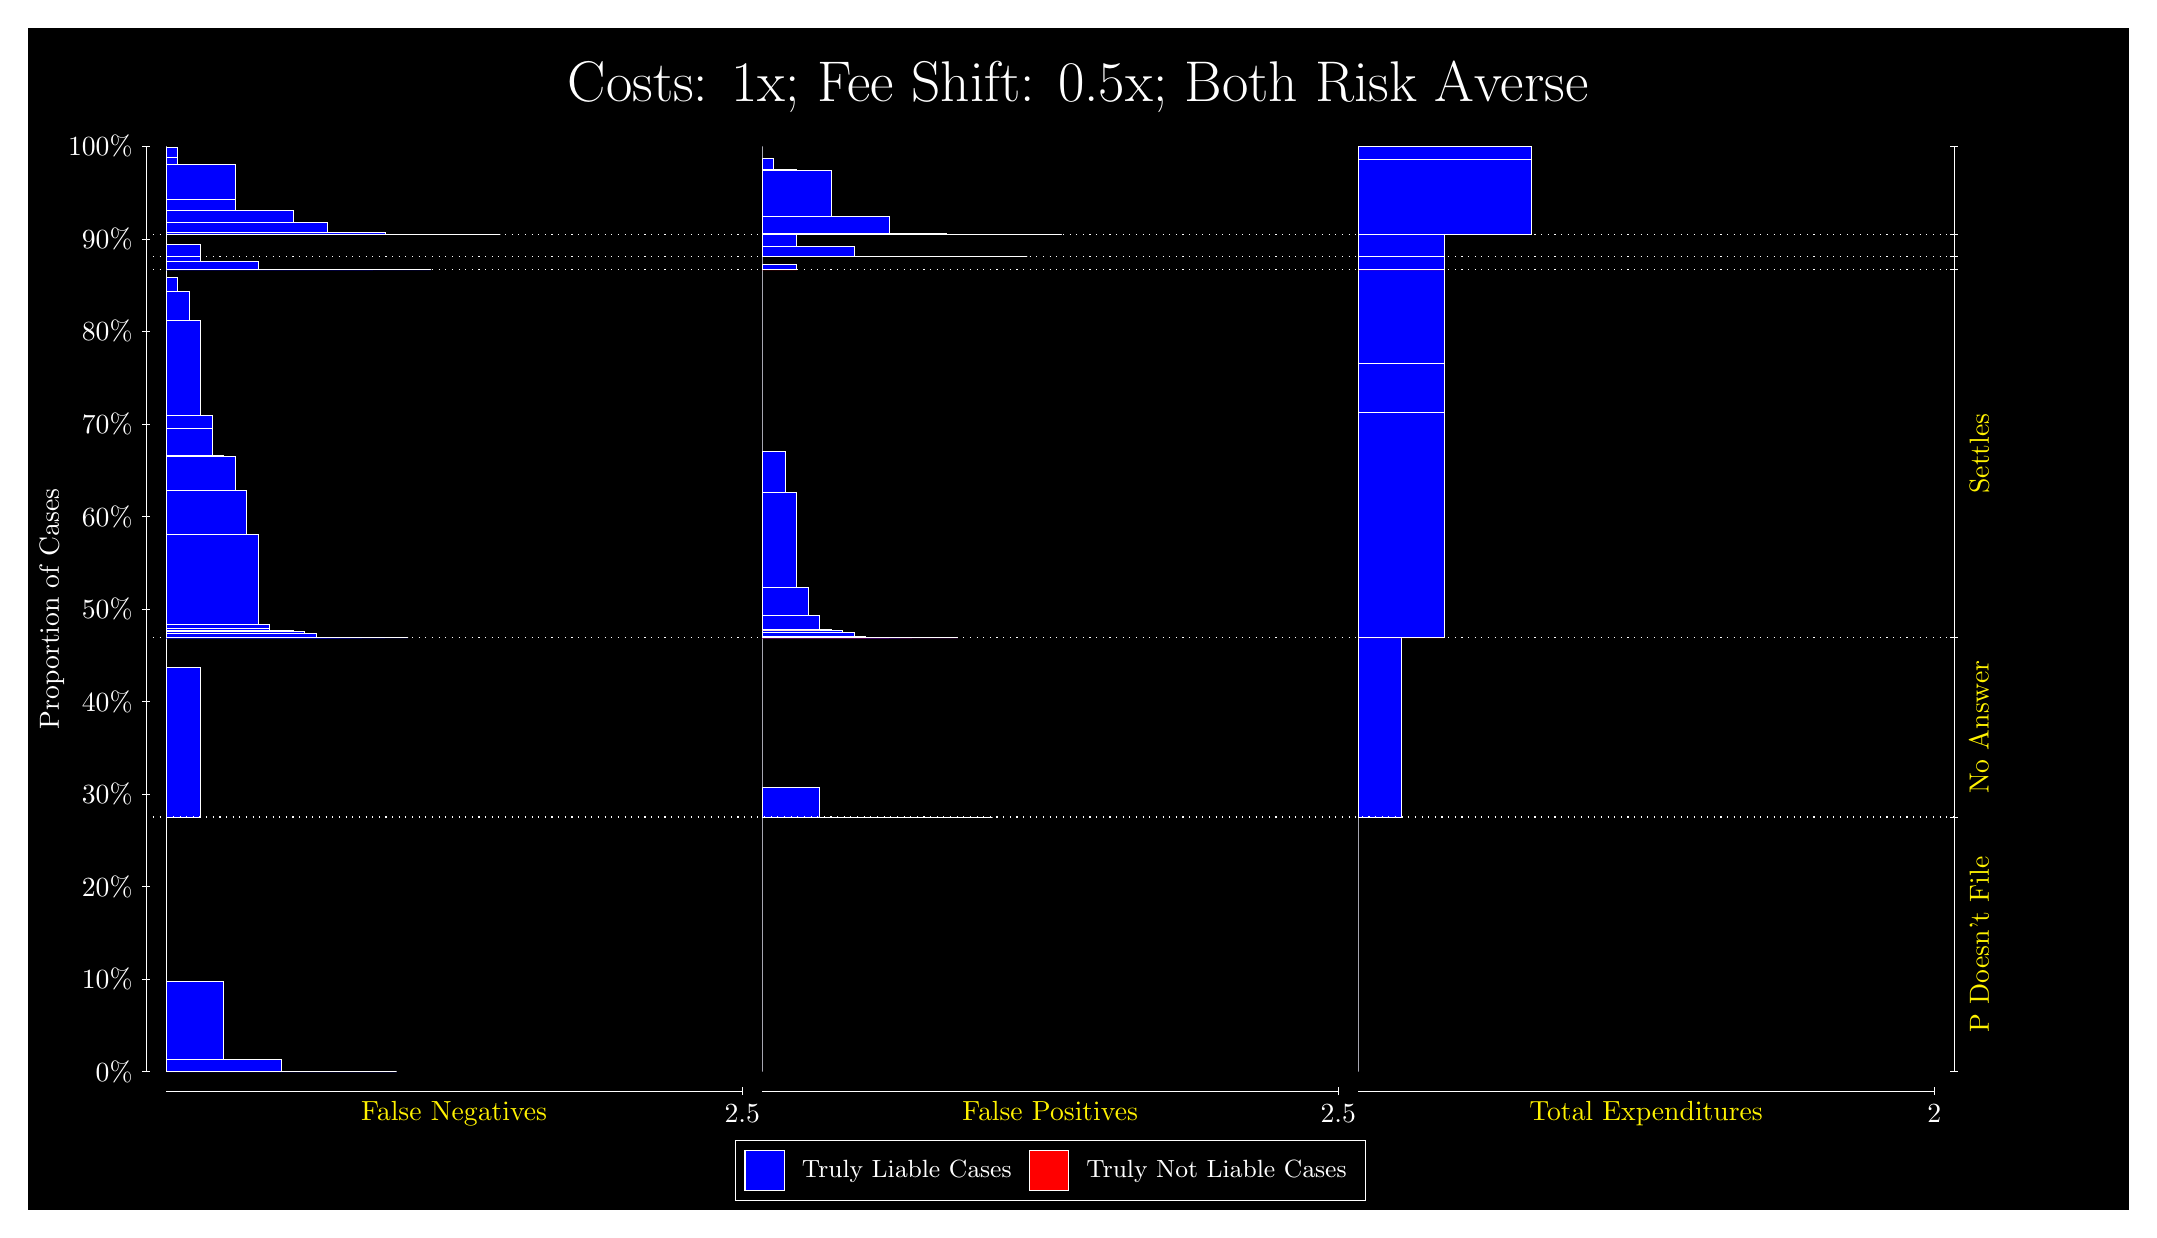
\begin{tikzpicture}
\draw[fill=black] (0,0) rectangle (26.667,15);
\draw[text=white] (0,13.5) rectangle (26.667,15) node[midway] {\huge Costs: 1x; Fee Shift: 0.5x; Both Risk Averse};
\draw[white, very thin] (1.5,1.75) -- (1.5,13.5);
\node[rotate=90, text=white, anchor=center] at (0.3, 7.625) {Proportion of Cases};
\draw[white, very thin] (1.45,1.75) -- (1.55,1.75);
\node[text=white, anchor=east] at (1.45, 1.75) {0\%};
\draw[white, very thin] (1.45,2.925) -- (1.55,2.925);
\node[text=white, anchor=east] at (1.45, 2.925) {10\%};
\draw[white, very thin] (1.45,4.1) -- (1.55,4.1);
\node[text=white, anchor=east] at (1.45, 4.1) {20\%};
\draw[white, very thin] (1.45,5.275) -- (1.55,5.275);
\node[text=white, anchor=east] at (1.45, 5.275) {30\%};
\draw[white, very thin] (1.45,6.45) -- (1.55,6.45);
\node[text=white, anchor=east] at (1.45, 6.45) {40\%};
\draw[white, very thin] (1.45,7.625) -- (1.55,7.625);
\node[text=white, anchor=east] at (1.45, 7.625) {50\%};
\draw[white, very thin] (1.45,8.8) -- (1.55,8.8);
\node[text=white, anchor=east] at (1.45, 8.8) {60\%};
\draw[white, very thin] (1.45,9.975) -- (1.55,9.975);
\node[text=white, anchor=east] at (1.45, 9.975) {70\%};
\draw[white, very thin] (1.45,11.15) -- (1.55,11.15);
\node[text=white, anchor=east] at (1.45, 11.15) {80\%};
\draw[white, very thin] (1.45,12.325) -- (1.55,12.325);
\node[text=white, anchor=east] at (1.45, 12.325) {90\%};
\draw[white, very thin] (1.45,13.5) -- (1.55,13.5);
\node[text=white, anchor=east] at (1.45, 13.5) {100\%};

\draw[white, very thin] (24.457,1.75) -- (24.457,13.5);
\draw[white, very thin] (24.407,1.75) -- (24.507,1.75);
\node[anchor=west] at (24.407, 1.75) {};
\draw[white, very thin] (24.407,4.9819) -- (24.507,4.9819);
\node[anchor=west] at (24.407, 4.9819) {};
\draw[white, very thin] (24.407,7.2617) -- (24.507,7.2617);
\node[anchor=west] at (24.407, 7.2617) {};
\draw[white, very thin] (24.407,11.935) -- (24.507,11.935);
\node[anchor=west] at (24.407, 11.935) {};
\draw[white, very thin] (24.407,12.101) -- (24.507,12.101);
\node[anchor=west] at (24.407, 12.101) {};
\draw[white, very thin] (24.407,12.385) -- (24.507,12.385);
\node[anchor=west] at (24.407, 12.385) {};
\draw[white, very thin] (24.407,13.5) -- (24.507,13.5);
\node[anchor=west] at (24.407, 13.5) {};

\draw[white, very thin, fill=blue] (1.75,1.75) rectangle (4.6775,1.75);
\draw[white, very thin, fill=blue] (1.75,1.75) rectangle (3.9457,1.7512);
\draw[white, very thin, fill=blue] (1.75,1.7512) rectangle (3.2138,1.8999);
\draw[white, very thin, fill=blue] (1.75,1.8999) rectangle (2.4819,2.9022);
\draw[white, very thin, fill=red] (1.75,2.9022) rectangle (1.75,2.9022);
\draw[white, very thin, fill=blue] (1.75,2.9022) rectangle (1.75,4.9819);
\draw[white, very thin, fill=blue] (1.75,4.9819) rectangle (2.1891,6.8887);
\draw[white, very thin, fill=red] (1.75,6.8887) rectangle (1.75,6.8887);
\draw[white, very thin, fill=blue] (1.75,6.8887) rectangle (1.75,7.2617);
\draw[white, very thin, fill=blue] (1.75,7.2617) rectangle (4.8239,7.2617);
\draw[white, very thin, fill=blue] (1.75,7.2617) rectangle (4.5312,7.2617);
\draw[white, very thin, fill=blue] (1.75,7.2617) rectangle (4.2384,7.2617);
\draw[white, very thin, fill=blue] (1.75,7.2617) rectangle (4.092,7.2617);
\draw[white, very thin, fill=blue] (1.75,7.2617) rectangle (3.9457,7.2617);
\draw[white, very thin, fill=blue] (1.75,7.2617) rectangle (3.7993,7.2618);
\draw[white, very thin, fill=blue] (1.75,7.2618) rectangle (3.6529,7.3149);
\draw[white, very thin, fill=blue] (1.75,7.3149) rectangle (3.5065,7.3353);
\draw[white, very thin, fill=blue] (1.75,7.3353) rectangle (3.3602,7.3524);
\draw[white, very thin, fill=blue] (1.75,7.3524) rectangle (3.2138,7.3527);
\draw[white, very thin, fill=blue] (1.75,7.3527) rectangle (3.0674,7.3787);
\draw[white, very thin, fill=blue] (1.75,7.3787) rectangle (3.0674,7.4258);
\draw[white, very thin, fill=blue] (1.75,7.4258) rectangle (2.921,8.5727);
\draw[white, very thin, fill=blue] (1.75,8.5727) rectangle (2.7746,9.1353);
\draw[white, very thin, fill=blue] (1.75,9.1353) rectangle (2.6283,9.5644);
\draw[white, very thin, fill=blue] (1.75,9.5644) rectangle (2.4819,9.5737);
\draw[white, very thin, fill=blue] (1.75,9.5737) rectangle (2.3355,9.9209);
\draw[white, very thin, fill=blue] (1.75,9.9209) rectangle (2.3355,10.088);
\draw[white, very thin, fill=blue] (1.75,10.088) rectangle (2.1891,11.297);
\draw[white, very thin, fill=blue] (1.75,11.297) rectangle (2.0428,11.657);
\draw[white, very thin, fill=blue] (1.75,11.657) rectangle (1.8964,11.836);
\draw[white, very thin, fill=blue] (1.75,11.836) rectangle (1.75,11.836);
\draw[white, very thin, fill=red] (1.75,11.836) rectangle (1.75,11.836);
\draw[white, very thin, fill=blue] (1.75,11.836) rectangle (1.75,11.935);
\draw[white, very thin, fill=blue] (1.75,11.935) rectangle (5.1167,11.935);
\draw[white, very thin, fill=blue] (1.75,11.935) rectangle (4.3848,11.935);
\draw[white, very thin, fill=blue] (1.75,11.935) rectangle (3.6529,11.938);
\draw[white, very thin, fill=blue] (1.75,11.938) rectangle (2.921,12.035);
\draw[white, very thin, fill=blue] (1.75,12.035) rectangle (2.1891,12.101);
\draw[white, very thin, fill=red] (1.75,12.101) rectangle (1.75,12.101);
\draw[white, very thin, fill=blue] (1.75,12.101) rectangle (2.1891,12.253);
\draw[white, very thin, fill=red] (1.75,12.253) rectangle (1.75,12.253);
\draw[white, very thin, fill=blue] (1.75,12.253) rectangle (1.75,12.385);
\draw[white, very thin, fill=blue] (1.75,12.385) rectangle (5.9949,12.385);
\draw[white, very thin, fill=blue] (1.75,12.385) rectangle (5.2631,12.386);
\draw[white, very thin, fill=blue] (1.75,12.386) rectangle (4.8239,12.386);
\draw[white, very thin, fill=blue] (1.75,12.386) rectangle (4.5312,12.407);
\draw[white, very thin, fill=blue] (1.75,12.407) rectangle (4.092,12.407);
\draw[white, very thin, fill=blue] (1.75,12.407) rectangle (3.7993,12.541);
\draw[white, very thin, fill=blue] (1.75,12.541) rectangle (3.3602,12.682);
\draw[white, very thin, fill=blue] (1.75,12.682) rectangle (3.0674,12.691);
\draw[white, very thin, fill=blue] (1.75,12.691) rectangle (2.6283,12.831);
\draw[white, very thin, fill=blue] (1.75,12.831) rectangle (2.6283,13.276);
\draw[white, very thin, fill=blue] (1.75,13.276) rectangle (2.3355,13.276);
\draw[white, very thin, fill=blue] (1.75,13.276) rectangle (1.8964,13.355);
\draw[white, very thin, fill=blue] (1.75,13.355) rectangle (1.8964,13.487);
\draw[white, very thin, fill=red] (1.75,13.487) rectangle (1.75,13.487);
\draw[white, very thin, fill=blue] (1.75,13.487) rectangle (1.75,13.5);
\draw[white, very thin, fill=red] (9.3189,1.75) rectangle (9.3189,1.75);
\draw[white, very thin, fill=blue] (9.3189,1.75) rectangle (9.3189,4.9819);
\draw[white, very thin, fill=red] (9.3189,4.9819) rectangle (12.246,4.9819);
\draw[white, very thin, fill=blue] (9.3189,4.9819) rectangle (12.246,4.9819);
\draw[white, very thin, fill=blue] (9.3189,4.9819) rectangle (11.515,4.9819);
\draw[white, very thin, fill=blue] (9.3189,4.9819) rectangle (10.783,4.9849);
\draw[white, very thin, fill=blue] (9.3189,4.9849) rectangle (10.051,5.3549);
\draw[white, very thin, fill=blue] (9.3189,5.3549) rectangle (9.3189,7.2617);
\draw[white, very thin, fill=red] (9.3189,7.2617) rectangle (11.807,7.2617);
\draw[white, very thin, fill=blue] (9.3189,7.2617) rectangle (11.807,7.2617);
\draw[white, very thin, fill=red] (9.3189,7.2617) rectangle (11.222,7.2617);
\draw[white, very thin, fill=blue] (9.3189,7.2617) rectangle (11.222,7.2618);
\draw[white, very thin, fill=blue] (9.3189,7.2618) rectangle (11.075,7.2618);
\draw[white, very thin, fill=red] (9.3189,7.2618) rectangle (10.929,7.2618);
\draw[white, very thin, fill=blue] (9.3189,7.2618) rectangle (10.929,7.2618);
\draw[white, very thin, fill=red] (9.3189,7.2618) rectangle (10.636,7.2618);
\draw[white, very thin, fill=blue] (9.3189,7.2618) rectangle (10.636,7.2747);
\draw[white, very thin, fill=blue] (9.3189,7.2747) rectangle (10.49,7.3322);
\draw[white, very thin, fill=red] (9.3189,7.3322) rectangle (10.344,7.3322);
\draw[white, very thin, fill=blue] (9.3189,7.3322) rectangle (10.344,7.3601);
\draw[white, very thin, fill=blue] (9.3189,7.3601) rectangle (10.197,7.3604);
\draw[white, very thin, fill=red] (9.3189,7.3604) rectangle (10.051,7.3604);
\draw[white, very thin, fill=blue] (9.3189,7.3604) rectangle (10.051,7.5389);
\draw[white, very thin, fill=blue] (9.3189,7.5389) rectangle (9.9044,7.8988);
\draw[white, very thin, fill=blue] (9.3189,7.8988) rectangle (9.758,9.1087);
\draw[white, very thin, fill=blue] (9.3189,9.1087) rectangle (9.6116,9.6225);
\draw[white, very thin, fill=blue] (9.3189,9.6225) rectangle (9.4652,9.6319);
\draw[white, very thin, fill=blue] (9.3189,9.6319) rectangle (9.3189,11.935);
\draw[white, very thin, fill=red] (9.3189,11.935) rectangle (9.758,11.935);
\draw[white, very thin, fill=blue] (9.3189,11.935) rectangle (9.758,12);
\draw[white, very thin, fill=blue] (9.3189,12) rectangle (9.3189,12.101);
\draw[white, very thin, fill=red] (9.3189,12.101) rectangle (12.686,12.101);
\draw[white, very thin, fill=blue] (9.3189,12.101) rectangle (12.686,12.101);
\draw[white, very thin, fill=blue] (9.3189,12.101) rectangle (11.954,12.101);
\draw[white, very thin, fill=blue] (9.3189,12.101) rectangle (11.222,12.102);
\draw[white, very thin, fill=blue] (9.3189,12.102) rectangle (10.49,12.233);
\draw[white, very thin, fill=blue] (9.3189,12.233) rectangle (9.758,12.385);
\draw[white, very thin, fill=red] (9.3189,12.385) rectangle (13.125,12.385);
\draw[white, very thin, fill=blue] (9.3189,12.385) rectangle (13.125,12.385);
\draw[white, very thin, fill=red] (9.3189,12.385) rectangle (12.393,12.385);
\draw[white, very thin, fill=blue] (9.3189,12.385) rectangle (12.393,12.385);
\draw[white, very thin, fill=red] (9.3189,12.385) rectangle (11.661,12.385);
\draw[white, very thin, fill=blue] (9.3189,12.385) rectangle (11.661,12.398);
\draw[white, very thin, fill=red] (9.3189,12.398) rectangle (11.222,12.398);
\draw[white, very thin, fill=blue] (9.3189,12.398) rectangle (11.222,12.398);
\draw[white, very thin, fill=red] (9.3189,12.398) rectangle (10.929,12.398);
\draw[white, very thin, fill=blue] (9.3189,12.398) rectangle (10.929,12.609);
\draw[white, very thin, fill=red] (9.3189,12.609) rectangle (10.49,12.609);
\draw[white, very thin, fill=blue] (9.3189,12.609) rectangle (10.49,12.609);
\draw[white, very thin, fill=blue] (9.3189,12.609) rectangle (10.197,13.195);
\draw[white, very thin, fill=blue] (9.3189,13.195) rectangle (9.758,13.201);
\draw[white, very thin, fill=red] (9.3189,13.201) rectangle (9.758,13.201);
\draw[white, very thin, fill=blue] (9.3189,13.201) rectangle (9.758,13.204);
\draw[white, very thin, fill=blue] (9.3189,13.204) rectangle (9.4652,13.344);
\draw[white, very thin, fill=blue] (9.3189,13.344) rectangle (9.3189,13.5);
\draw[white, very thin, fill=red] (16.888,1.75) rectangle (16.888,1.75);
\draw[white, very thin, fill=blue] (16.888,1.75) rectangle (16.888,4.9819);
\draw[white, very thin, fill=red] (16.888,4.9819) rectangle (17.437,4.9819);
\draw[white, very thin, fill=blue] (16.888,4.9819) rectangle (17.437,7.2617);
\draw[white, very thin, fill=red] (16.888,7.2617) rectangle (17.986,7.2617);
\draw[white, very thin, fill=blue] (16.888,7.2617) rectangle (17.986,10.121);
\draw[white, very thin, fill=red] (16.888,10.121) rectangle (17.986,10.121);
\draw[white, very thin, fill=blue] (16.888,10.121) rectangle (17.986,10.745);
\draw[white, very thin, fill=red] (16.888,10.745) rectangle (17.986,10.745);
\draw[white, very thin, fill=blue] (16.888,10.745) rectangle (17.986,11.935);
\draw[white, very thin, fill=red] (16.888,11.935) rectangle (17.986,11.935);
\draw[white, very thin, fill=blue] (16.888,11.935) rectangle (17.986,12.101);
\draw[white, very thin, fill=red] (16.888,12.101) rectangle (17.986,12.101);
\draw[white, very thin, fill=blue] (16.888,12.101) rectangle (17.986,12.385);
\draw[white, very thin, fill=red] (16.888,12.385) rectangle (19.083,12.385);
\draw[white, very thin, fill=blue] (16.888,12.385) rectangle (19.083,13.335);
\draw[white, very thin, fill=red] (16.888,13.335) rectangle (19.083,13.335);
\draw[white, very thin, fill=blue] (16.888,13.335) rectangle (19.083,13.5);
\draw[white, dotted] (1.5,4.9819) -- (24.457,4.9819);
\draw[white, dotted] (1.5,7.2617) -- (24.457,7.2617);
\draw[white, dotted] (1.5,11.935) -- (24.457,11.935);
\draw[white, dotted] (1.5,12.101) -- (24.457,12.101);
\draw[white, dotted] (1.5,12.385) -- (24.457,12.385);
\draw[white, very thin] (1.75,1.5) -- (9.0689,1.5);
\node[text=yellow, anchor=north] at (5.4094, 1.5) {False Negatives};
\draw[white, very thin] (9.0689,1.45) -- (9.0689,1.55);
\node[text=white, anchor=north] at (9.0689, 1.45) {2.5};

\draw[white, very thin] (9.3189,1.5) -- (16.638,1.5);
\node[text=yellow, anchor=north] at (12.978, 1.5) {False Positives};
\draw[white, very thin] (16.638,1.45) -- (16.638,1.55);
\node[text=white, anchor=north] at (16.638, 1.45) {2.5};

\draw[white, very thin] (16.888,1.5) -- (24.207,1.5);
\node[text=yellow, anchor=north] at (20.547, 1.5) {Total Expenditures};
\draw[white, very thin] (24.207,1.45) -- (24.207,1.55);
\node[text=white, anchor=north] at (24.207, 1.45) {2};

\node[text=yellow, centered, rotate=90] at (24.777, 3.366) {P Doesn't File};
\node[text=yellow, centered, rotate=90] at (24.777, 6.1218) {No Answer};
\node[text=yellow, centered, rotate=90] at (24.777, 9.5981) {Settles};




\draw (12.978300999999998,1.5) node[draw=none] (baseCoordinate) {};
\begin{scope}[align=center]
        \matrix[scale=0.5, draw=white, below=0.5cm of baseCoordinate, nodes={draw}, column sep=0.1cm]{
            \node[rectangle, draw, minimum width=0.5cm, minimum height=0.5cm, fill=blue] {}; &
            \node[draw=none, font=\small, text=white] (B) {Truly Liable Cases}; &
            \node[rectangle, draw, minimum width=0.5cm, minimum height=0.5cm, fill=red] {}; &
            \node[draw=none, font=\small, text=white] (B) {Truly Not Liable Cases}; \\
            };
\end{scope}

\end{tikzpicture}
\end{document}